% A seção de Metodologia explica aos leitores quais procedimentos, abordagens, desenhos e tratamento realizamos na pesquisa, o que permitirá replicar os estudos, entender a linearidade entre a abordagem dos objetivos e os resultados obtidos, determinar sua adequação e relevância e evidenciar qualquer viés na maneira como o estudo foi elaborado e realizado. Em outras palavras, é uma estrutura contextual que apresenta um caminho lógico para responder a perguntas que você levanta no início de sua tese ou artigo. 

% É importante que nesta seção, você descreva todas as ferramentas e tecnologias utilizadas para o desenvolvimento da sua pesquisa \cite{boulic:91}. Lembre-se de detalhar para que serve cada ferramenta e tecnologia e o motivo da sua escolha.

Neste projeto, será desenvolvido um sistema de auditoria de conteúdo \textit{Web}, utilizando técnicas de PLN, que proporcione a identificacão e o bloqueio de sites acessados no âmbito escolar que contenham contextos discriminatórios. Utilizando IA, por meio do Processamento de Linguagem Natural (PLN). Quando um aluno acessar um site na \textit{Web}, o programa, escaneará todo o conteúdo da página em busca de contexto de discriminação. Caso haja algo, o programa atuará por meio de um proxy, para bloquear o site em toda a rede. Caso contrário, o site será aberto normalmente no navegador.
O proxy é um aplicativo do servidor que atua na intermediação entre um cliente que solicita um recurso e um servidor que o fornece, portanto, ele é capaz de monitorar e controlar o acesso a sites em uma rede. 

Para as primeiras implementações do sistema de bloqueio automatizado, a tecnologia utilizada no o back-end será Python, escolhida pela sua vasta gama de bibliotecas que auxiliarão no tratamento e manipulação do conteúdo das páginas. O Ambiente de Desenvolvimento Integrado (IDE) escolhido para manipular a linguagem foi o Visual Studio Code, notável pela sua flexibilidade e suporte de diversas extensões, o que auxiliam no processo de codificação.

O fluxo do sistema respresentado no \Cref{fcht:fluxograma} se inicia quando o cliente faz uma solicitação ao servidor/proxy (Etapa A). Para atuar como servidor, utilizaremos o Ubuntu, uma das distribuições mais populares do sistema operacional Linux. É conhecido por sua facilidade de uso, estabilidade e segurança.\textcite{ubuntu-desktop} Nele, será instalado um \textit{Software} de Proxy conhecido como Squid, que permite monitorar as páginas acessadas pelos computadores conectados, bem como impede o acesso a determinados \textit{websites}.\cite{squid-cache}, e atua como intermediário entre o cliente e a internet (Etapa B). Em seguida, a solicitação do cliente é enviada à internet para buscar o conteúdo requisitado (Etapa C).
A cada solicitação, o sistema registra informações de acesso, como data, hora, IP da máquina e URL do site acessado, e armazena esses dados no arquivo access.log do servidor (Etapa D).

Na etapa seguinte, o módulo indexador registra no banco de dados as informações do acesso mais recente registrado no access.log (Etapa E). No projeto será implementado o modelo NoSQL. A escolha pelo MongoDB se deve pela sua orientação de documentos do tipo JavaScript Object Notation (JSON), que é um formato leve e fácil de usar para armazenar e transportar dados. O MongoDB possui capacidade de lidar com grandes volumes de dados não estruturados de maneira eficaz, além de sua alta disponibilidade e suporte à replicação, fornecendo garantia a continuidade do sistema em caso de falhas. 
A finalidade dessa etapa é aprimorar a capacidade de monitoramento do sistema. Os dados registrados incluem o caminho do arquivo com o conteúdo indexado (pathLocal), um indicador do tipo booleano que sinaliza se o acesso está bloqueado ou não (flag), a URL acessada (urlWeb) e o termo identificado que pode ter causado o bloqueio.

Posteriormente, o conteúdo é armazenado no banco de dados, e enviado para avaliação e classificação pelo Módulo de Inteligência Artificial (Etapa F). Nesse momento, a Inteligência Artificial (IA) identifica e classifica o conteúdo com base nos parâmetros estabelecidos (Etapa G). A IA desenvolvida neste projeto tem como foco principal identificar contextos discriminatórios em conteúdos acessados na internet, utilizando técnicas avançadas de PLN. O modelo foi construído com base na arquitetura BERT, uma tecnologia de aprendizado profunda desenvolvida pelo Google que permite a compreensão do contexto das palavras em um texto de forma bidirecional. Isso significa que o modelo analisa uma palavra considerando tanto o que vem antes quanto o que vem depois, garantindo maior precisão na interpretação semântica.

O treinamento da IA foi realizado utilizando o \textit{dataset} público \textit {Jigsaw Unintended Bias}, amplamente reconhecido em estudos relacionados à detecção de discurso de ódio. Este \textit{dataset} contém milhões de exemplos rotulados de comentários online e textos, além de que, ele inclui diversas categorias de discurso ofensivo, como toxicidade geral, insultos, ameaças, ataques à identidade, conteúdo obsceno e sexual explícito. Antes do treinamento, os dados passaram por etapas de pré-processamento, como limpeza textual e tokenização, que converte os textos em entradas numéricas compatíveis com o modelo BERT, permitindo que ele processe e aprenda padrões relevantes para a tarefa.

Com os resultados dessa análise, o sistema verifica o nível de toxidade do texto e o classifica em: Toxicity (tóxico), Severe Toxicity (severamente tóxico), Obscene (obsceno), Sexual Explicit (sexualmente explicito), Identity Attack (ataque de identidade), Threat (ameaça) e Insult (insulto). Caso o nível de toxidade (TOXITS) seja inferior a 50%, a solicitação retorna ao cliente, permitindo o acesso normal ao conteúdo (Etapa H).

Se o conteúdo for considerado tóxico, ou seja, com classificação superior a 50\%, ele é adicionado a uma lista de bloqueio no servidor denominada bloqueados.txt, impedindo acessos futuros ao mesmo conteúdo (Etapa I).

Além disso, após a classificação feita pelo Módulo IA, se o conteúdo for considerado tóxico, ele é encaminhado ao Módulo de Treinamento para aprimorar a IA. O conteúdo tóxico é utilizado no treinamento da IA sendo armazenado no banco de dados com informações de contexto, servindo como referência para futuras classificações. A Rede Neural Artificial (RNA) da IA é então atualizada com esses novos dados, permitindo a retroalimentação do sistema e garantindo que ele continue a evoluir e se adaptar, melhorando a eficiência na detecção e classificação de conteúdos potencialmente prejudiciais (Etapa J).

Por fim, quando uma URL é adicionada à lista de bloqueio ou o cliente solicita acesso a uma URL já bloqueada, o sistema exibe uma notificação informando que o acesso foi restrito devido ao alto nível de TOXITS (Etapa I).

\begin{flowchart}[H]
    \centering
    \caption{Resist}%
    \label{fcht:fluxograma}
    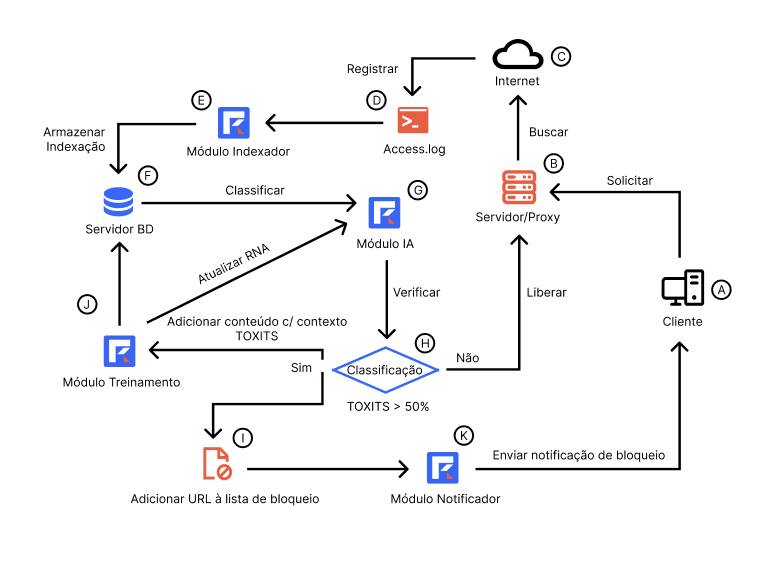
\includegraphics[scale=.68]{fluxograma}
    \SourceOrNote{Autoria Própria (2024)}
    \end{flowchart}